\begin{flushright} {\tiny {\color{gray} python\_codes/fieldstone\_125/text.tex}} \end{flushright}

%\lstinputlisting[language=bash,basicstyle=\small]{python_codes/fieldstone_125/keywords}

\begin{center}

\fbox{\textbf{\huge \color{teal} P}}
Code at \url{https://github.com/cedrict/fieldstone/tree/master/python_codes/fieldstone_125}
\end{center}

\par\noindent\rule{\textwidth}{0.4pt}

%--------------------------------------------------------------------------------------------

To quote Wikipedia\footnote{\url{https://en.wikipedia.org/wiki/Voronoi_diagram}}:
``In mathematics, a Voronoi diagram is a partition of a plane into regions close to each of a given set of objects. 
In the simplest case, these objects are just finitely many points in the plane (called seeds, sites, or generators). 
For each seed there is a corresponding region, called a Voronoi cell, consisting of all points of the plane closer to 
that seed than to any other. The Voronoi diagram of a set of points is dual to its Delaunay triangulation. ''

\Literature: \textcite{may12} (2012), \textcite{hust08b} (2008).

The domain is a 2D ({\python ndim=2}) or 3D ({\python ndim=3}) 
Cartesian box. A regular grid spans this domain with resolution 
$nelx \times nely$ or $nelx \times nely \times nelz$. 
In each cell $nmarker\_per\_dim^{ndim}$ markers are regularly placed. 
Finally $nvo$ seeds are randomly placed in the domain and wish to compute the Voronoi cell attached to 
each seed. There are three test cases in the code, differing only by the number of seeds (7,27,111 respectively).
The volume of each cell is also computed (based on the area assigned to each marker).

TODO: write a faster version which assigns a V cell to a marker using the cell number of its neighbour. 
Credit Henry and link to his thesis appendix.


%-----------------------------
\subsubsection*{Test \# 1}

\begin{center}
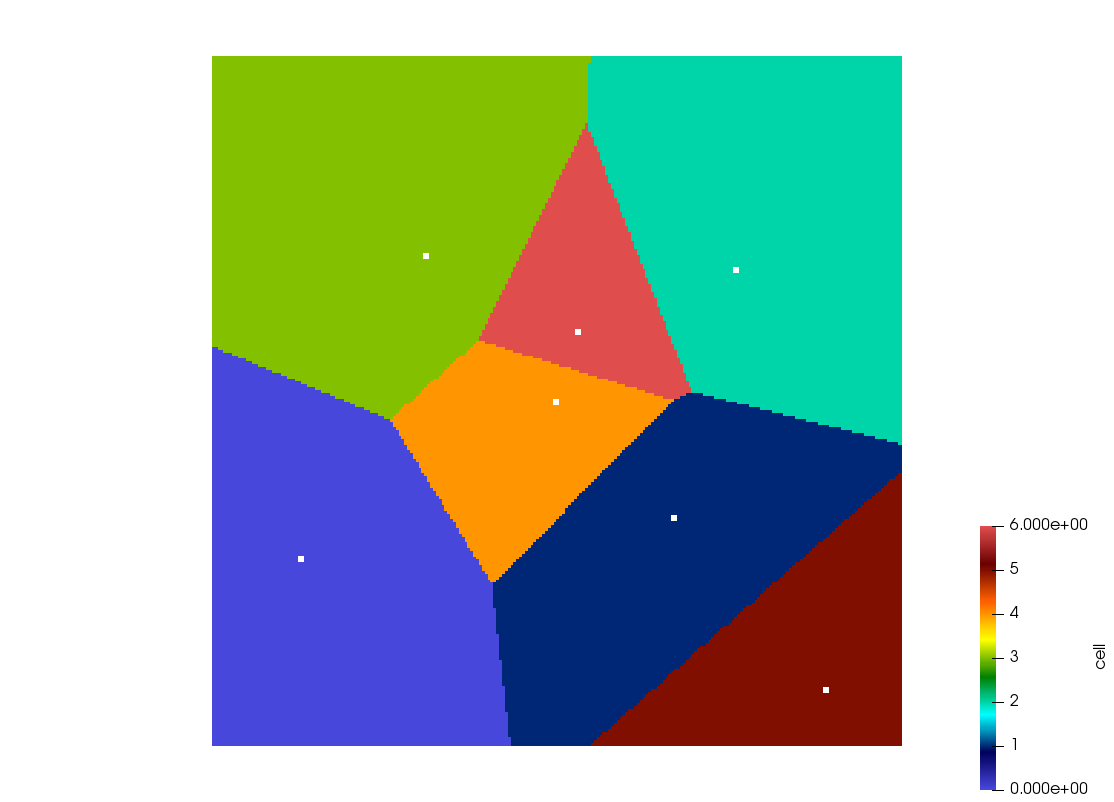
\includegraphics[width=6cm]{python_codes/fieldstone_125/results/diagram.png}\\
{\captionfont Example with 7 seeds.}
\end{center}


%-----------------------------
\subsubsection*{Test \# 2}

\begin{center}

\includegraphics[width=6cm]{python_codes/fieldstone_125/results/test2_a}

\includegraphics[width=6cm]{python_codes/fieldstone_125/results/test2_b}\\
{\captionfont Examples with two different sets of 27 random seeds in 2D.}
\end{center}

\begin{center}
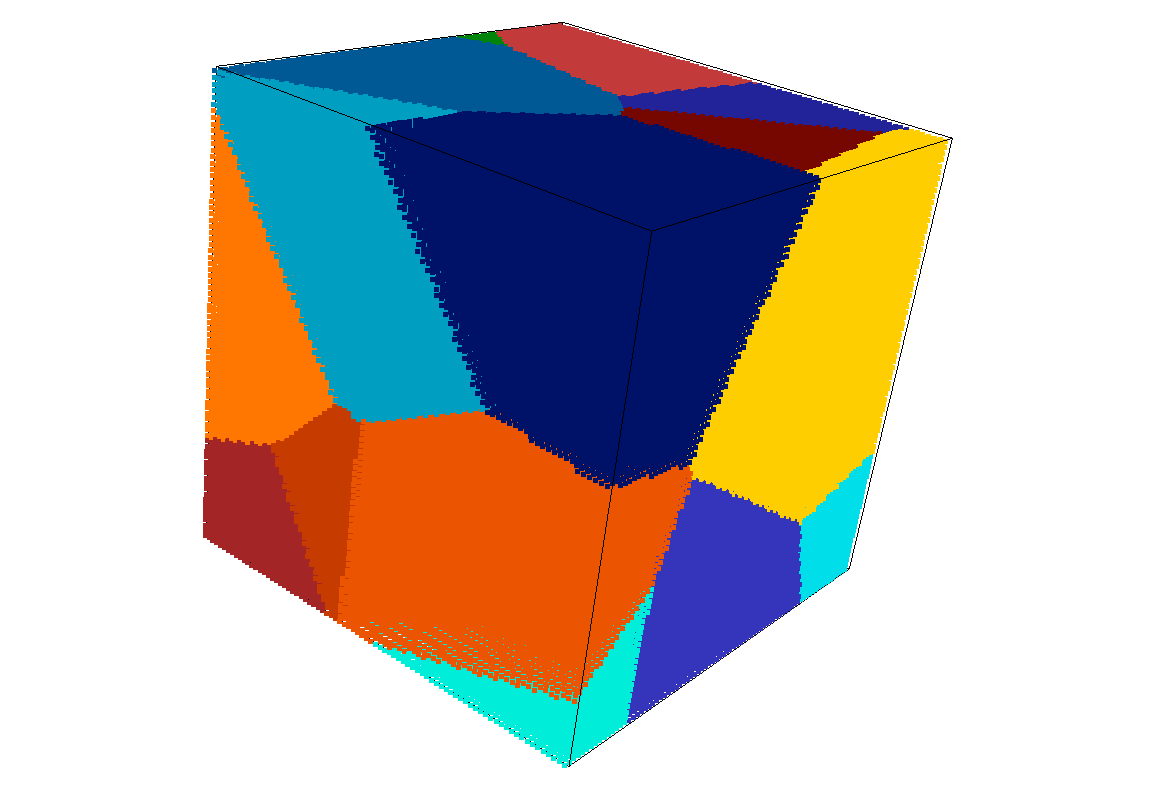
\includegraphics[width=6cm]{python_codes/fieldstone_125/results/test2_3Da}
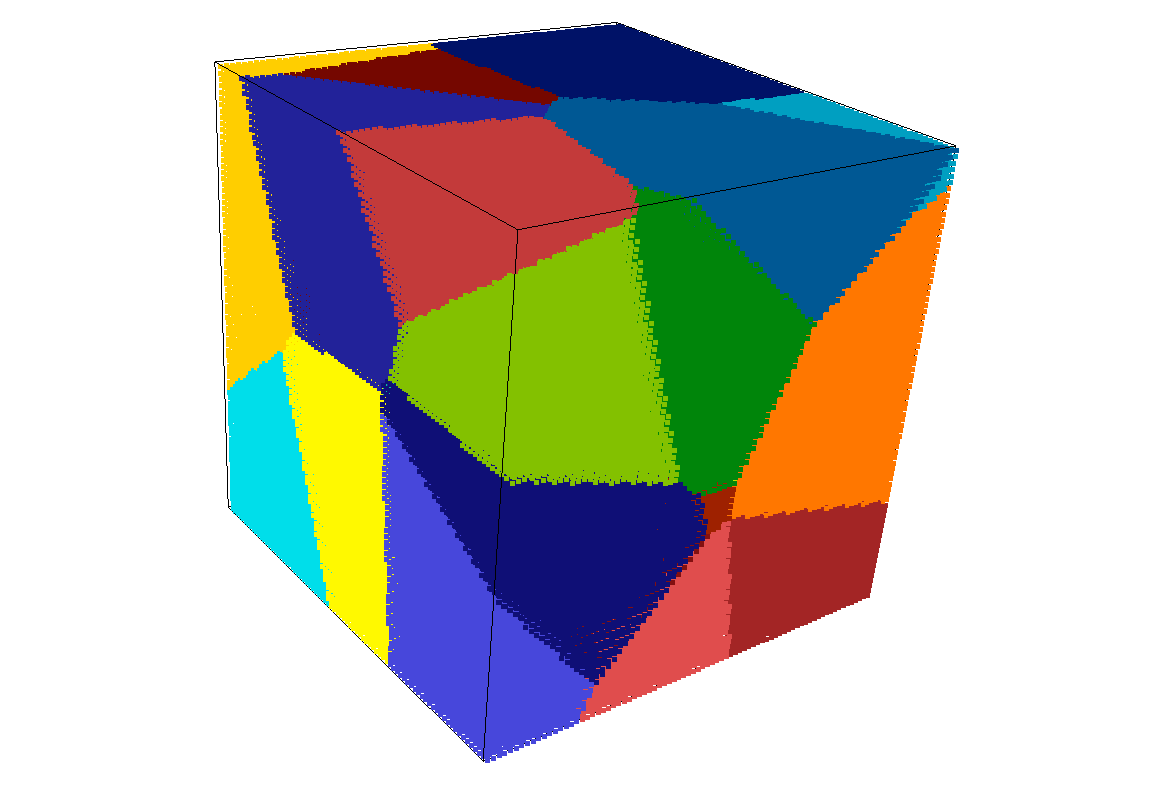
\includegraphics[width=6cm]{python_codes/fieldstone_125/results/test2_3Db}\\
{\captionfont Example with 27 random seeds in 2D (different views).}
\end{center}

%-----------------------------
\subsubsection*{Test \# 3}

\begin{center}
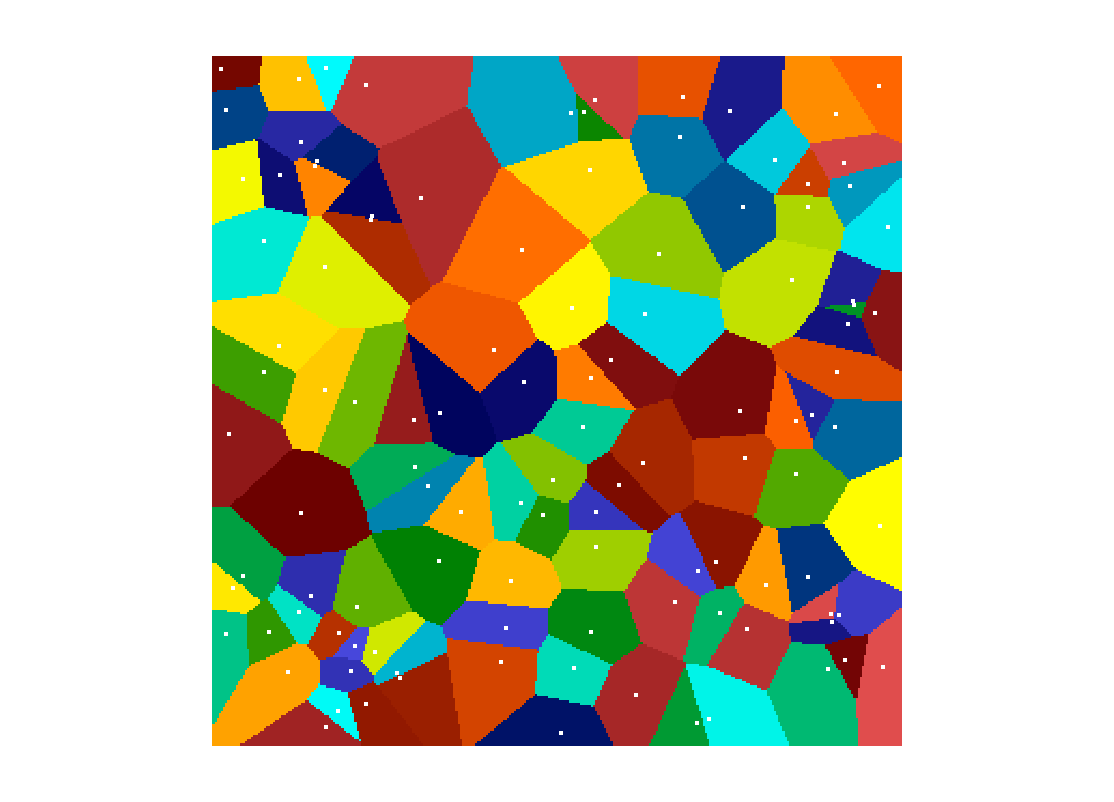
\includegraphics[width=6cm]{python_codes/fieldstone_125/results/test3}
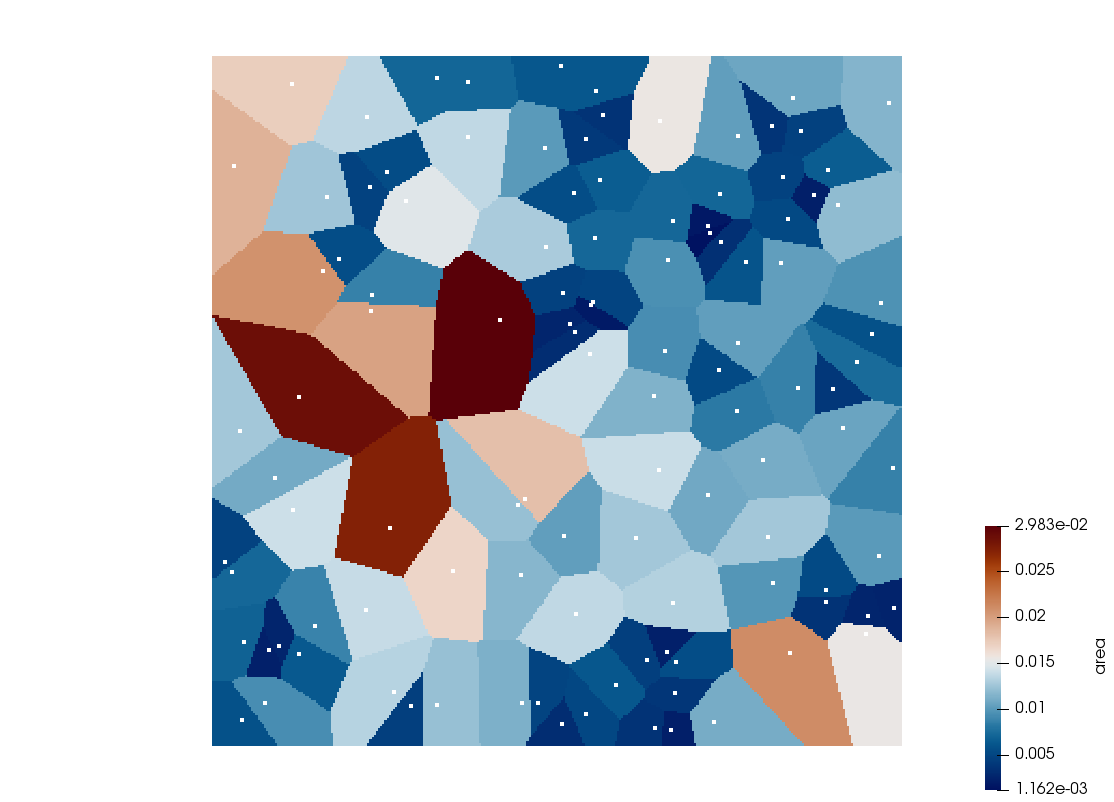
\includegraphics[width=6cm]{python_codes/fieldstone_125/results/test3_area}\\
{\captionfont Examples with 111 random seeds. Approx 310s.}
\end{center}

%-----------------------------
\subsubsection*{Test \# 4}

\begin{center}
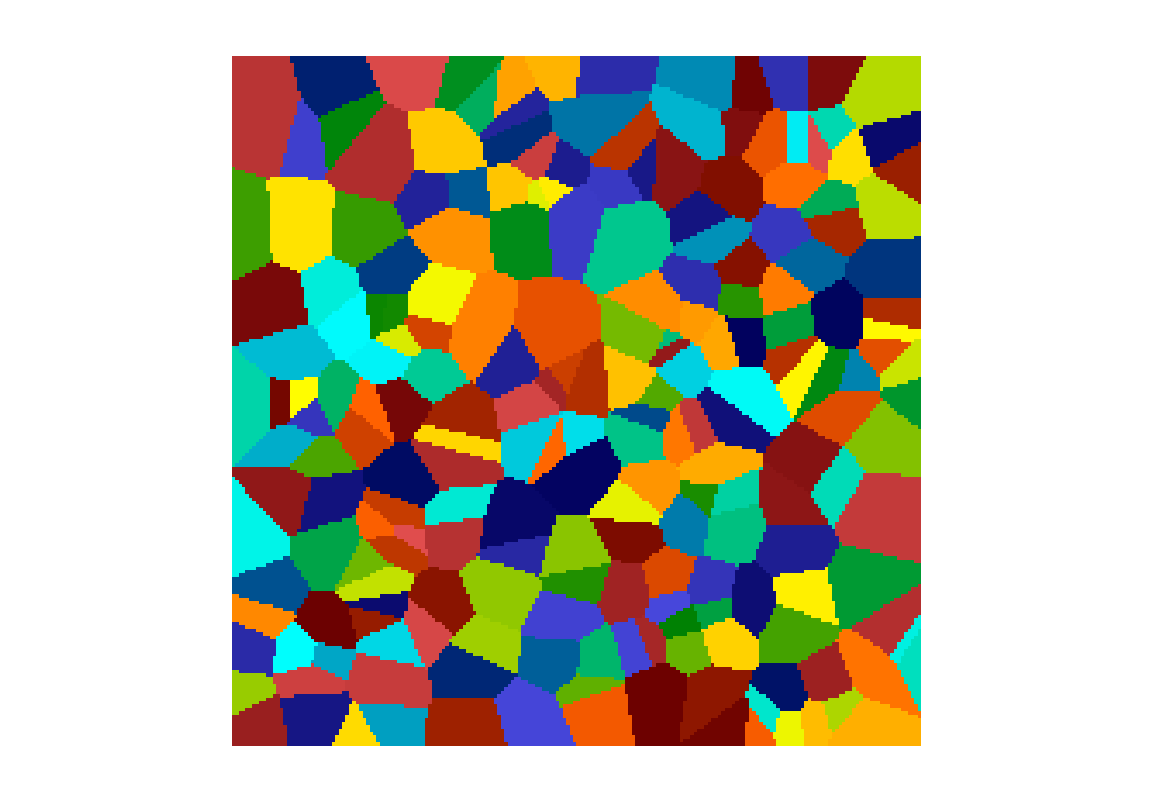
\includegraphics[width=6cm]{python_codes/fieldstone_125/results/test4a}
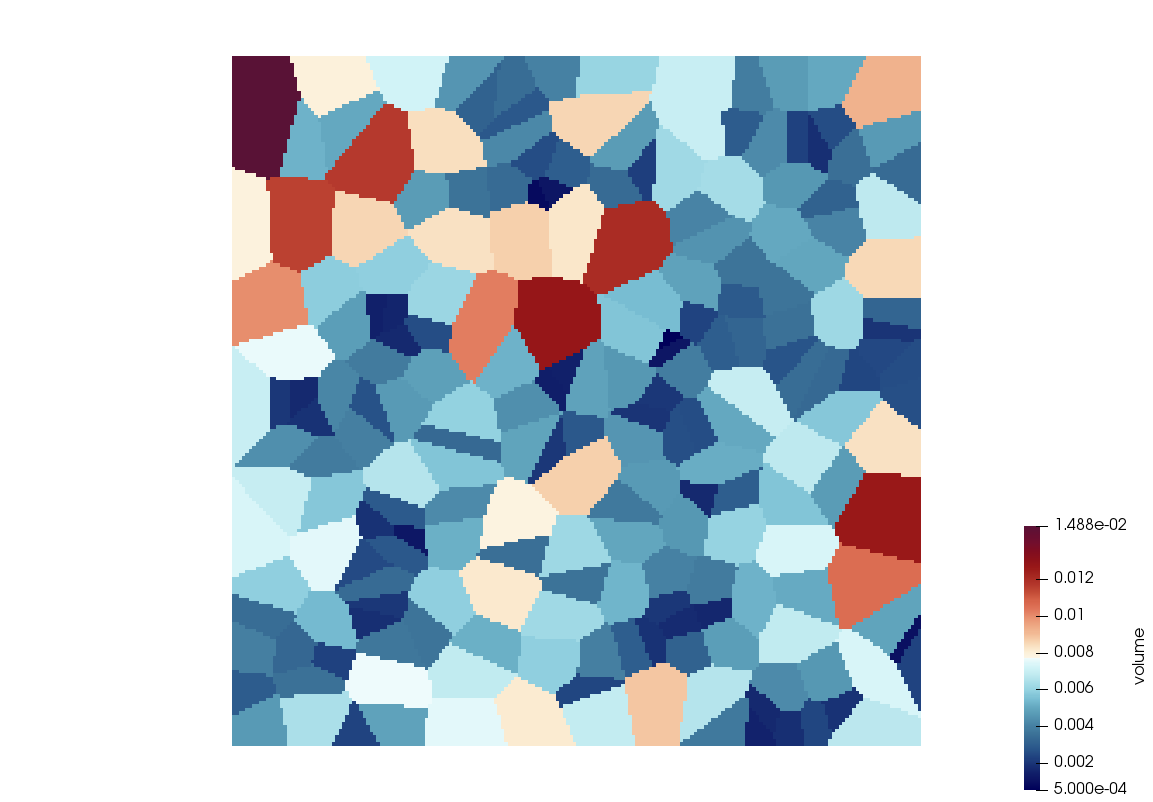
\includegraphics[width=6cm]{python_codes/fieldstone_125/results/test4b}\\
{\captionfont Examples with 40,000 markers and 213 random seeds. Approx 275s. }
\end{center}

%------------------------------------------------------------------------------
\noindent\rule{\textwidth}{1pt}

This is a completely different exercise. A swarm of points is generated in a 3D Cartesian 
domain using a random number generator for the coordinates.
The code computes the so-called Radial Distribution Function
\footnote{\url{https://en.wikipedia.org/wiki/Radial_distribution_function}}, 
which is describes how density varies as a function of distance from a reference particle. 
In simplest terms it is a measure of the probability of finding a particle at a distance of $r$ 
away from a given reference particle, relative to that for an ideal gas. 
The general algorithm involves determining how many particles are within a distance of $r$ and $r+dr$ away from a particle. 

The implemented algorithm is rather simple. Loop over all particles, and for each of them 
loop over the rest of the particles, compute the distance, find out in which bin of size $dr$ it belongs 
to and increase the count in that bin. We end up with the raw distribution.
Note that in order to avoid to count the same pair twice the second loop 
runs over 0 to i, and not 0 to nmarker (It also saves a lot of time!).
As explained on Wikipedia, one can also normalise it by $\rho 4\pi r^2 dr$, where $\rho$ is
the average density of points (number of points / volume). This yields the 
normalised rdf. 
Also note that points close to the sides of the domain are not 'seeing' the ones 
on the other side (no periodic conditions) so this is likely to alter the results.

\begin{center}
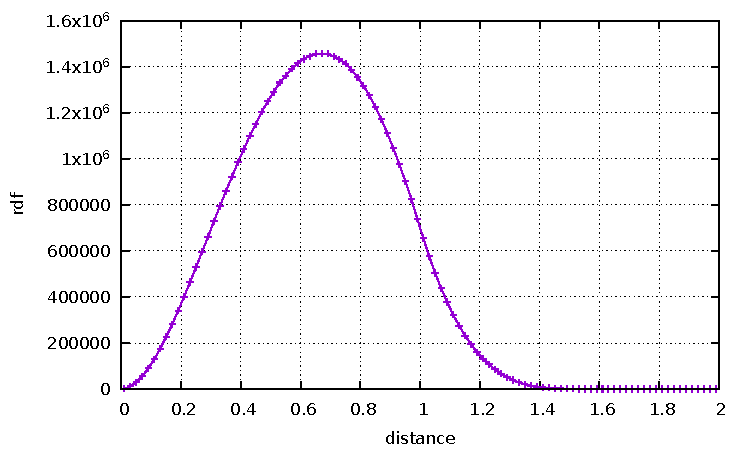
\includegraphics[width=7cm]{python_codes/fieldstone_125/results/rdf/rdf}
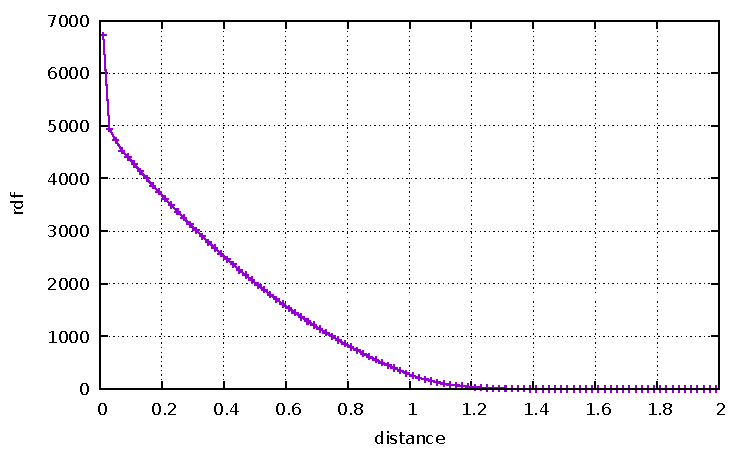
\includegraphics[width=7cm]{python_codes/fieldstone_125/results/rdf/rdf_normalised}\\
{\captionfont a }
\end{center}
 


















